
\section{Data}
\label{sec:data}

In this research, we use three data sources to build a monthly panel that covers our three pre-selected metropolitan areas. The raw Zillow and national FRED panel spans January~2000 to March~2026. The supervised complete-case sample begins in 2018 because the Zillow listing-side variables are unavailable before then and predictors are lagged. The OLS, XGBoost, and MLP models are trained on 168 complete pre-2023 observations and evaluated on 97 complete test observations (36 in San~Francisco, 36 in Austin, 25 in Cleveland). The ARIMA baseline is estimated separately by metro on the longer target-only ZHVI return history (back to January~2000) and then aligned to the same 97-observation supervised test grid for evaluation.

\subsection{Zillow Home Value Index}

Our first data source is the Zillow Home Value Index (ZHVI). This smoothed and seasonally adjusted variable quantifies the median home value for the middle price tier in each metropolitan area. The indicator is published monthly by Zillow Research and is available from January 2000 onward. We load this data source automatically in our notebook from Zillow's public static CSV URL.

In addition to the Home Value Index, we use three other real-time market activity variables published by Zillow Research: the monthly count of new listings, the median number of days a home sits on the market before going under contract, and the share of active listings that received a price reduction. These three variables impose a time constraint on the continuity of our dataset, as they are only available from 2018 onward. We therefore adjust our sample timeline to begin in that year.

Figure~\ref{fig:zhvi} shows the different paths for housing prices over the entire period in the three metros.

\begin{figure}[!htb]
\centering
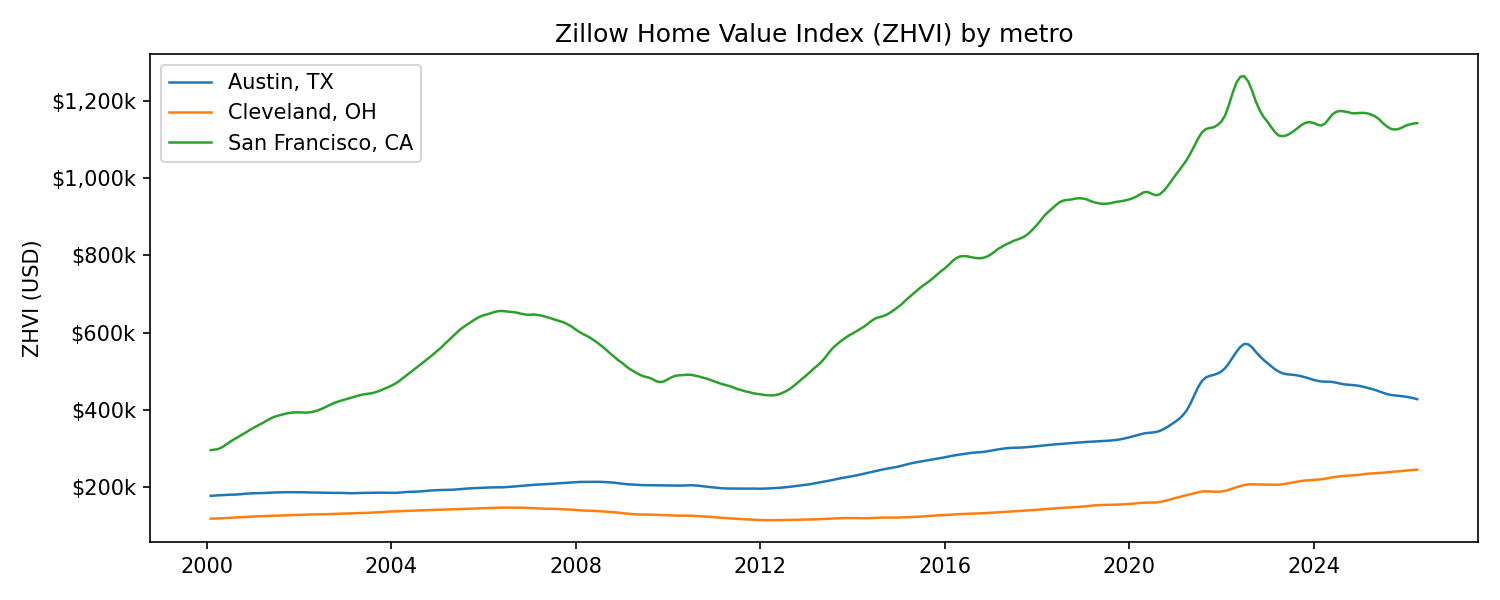
\includegraphics[width=0.68\textwidth]{zhvi_levels.png}
\caption{Zillow Home Value Index, by metro, January 2000 to March 2026. San Francisco and Austin experience steep price growth and increased volatility compared to Cleveland, whose path is more steady and less volatile.}
\label{fig:zhvi}
\end{figure}


\subsection{National Macroeconomic Indicators}

We selected five national economic indicators from the Federal Reserve Bank of St. Louis (FRED). These time series capture the key macroeconomic mechanisms through which monetary policy and credit conditions react to and affect local housing markets. First, the 30-year mortgage rate proxies buyer affordability and therefore housing demand. Second, the national unemployment rate reports labor market conditions. Third, the Consumer Price Index measures inflation and captures fluctuations in the real cost of housing. Fourth, housing starts measure new construction activity, which serves as a proxy for supply-side conditions. Finally, the St. Louis Fed Financial Stress Index captures credit-market conditions beyond the policy rate. We convert the weekly series into monthly averages to align them with the Zillow and unemployment indicators.

\subsection{Metro-Level Unemployment}

To adjust our approach to the metropolitan level, we use monthly, seasonally adjusted series that capture local labor market conditions that the national indicators cannot. Specifically, we include metro-specific unemployment series, as additional independent variables, from the Bureau of Labor Statistics Local Area Unemployment Statistics (LAUS). We retrieve them via FRED: series \texttt{SANF806URN} for San~Francisco, \texttt{AUST448URN} for Austin, and \texttt{CLEV439URN} for Cleveland.

Figure~\ref{fig:unrate} displays the unemployment trends for all three metros alongside the national average rate, demonstrating the differences in their labor markets over the sample period

\begin{figure}[!htb]
\centering

\includegraphics[width=0.68\textwidth]{unrate_metro.png}
\caption{Metro-level unemployment rates (LAUS, seasonally adjusted) versus the national unemployment rate (dashed), January 2000 to March 2026. San Francisco displays greater cyclical movements, whereas Cleveland sustains a steady but higher level of unemployment.}
\label{fig:unrate}
\end{figure}


\subsection{Sample Construction and Cleaning}

We merge the three data sources into a single dataframe in which each row corresponds to one observation per city per month, broadcasting the national macroeconomic indicators across all metros. Because the three Zillow listing-side variables are missing before 2018, we drop rows with missing values, which constrains the supervised modeling sample to 2018 onward. After cleaning, the supervised complete-case panel contains 168 training observations (pre-2023) and 97 test observations across the three metros (36 in San~Francisco, 36 in Austin, 25 in Cleveland). The ARIMA baseline does not require the lagged exogenous predictors, so it is estimated on the longer per-metro target-only history (back to 2000) and then evaluated on the same 97-observation supervised test grid for a strictly same-sample comparison. Figure~\ref{fig:missing} confirms that the Zillow listing-side variables are what constrain the start date of the supervised training window.

The smaller Cleveland test sample (25 observations versus 36 for the other two metros) is not driven by the Zillow listing-side variables. It reflects the fact that the extracted Cleveland LAUS metro unemployment series ends in December~2024 in our data pull, while the Zillow and national FRED series extend through March~2026. After the one-month lag is applied to \texttt{d\_unrate\_metro}, the last test month in which Cleveland passes the complete-case mask is January~2025.

\subsection{2024 ACS Variables (Descriptive Only)}

We also downloaded 2024 ACS 5-year metro-level variables --- median household income, median home value, and the rental vacancy rate --- for descriptive context. We do \emph{not} include them in the final model matrix because they are time-invariant within each of the three metros and are therefore perfectly collinear with the full set of metro fixed effects. The metro fixed effects already absorb these structural cross-metro differences (price level, income, vacancy regime), so adding the ACS variables would simply duplicate the dummies and make the design matrix rank-deficient.

\begin{figure}[!htb]
\centering

\includegraphics[width=0.68\textwidth]{missingness.png}
\caption{Share of missing observations per variable by year. Dark cells represent complete data; light cells indicate missing  values. The Zillow listing-side variables (new listings, days  pending, price cuts) are missing before 2018, which determines the effective start of the modeling sample.}
\label{fig:missing}
\end{figure}


Table~\ref{tab:summary} provides summary statistics of the relevant variables in the modeling sample by metropolitan area.

\begin{table}[h]
\centering
\small
\caption{Summary statistics by metropolitan area.
ZHVI is presented in thousands of US dollars. Log return is the monthly log return of ZHVI. Metro unemployment is the LAUS seasonally-adjusted rate expressed as a percentage. Listing-side variables (new listings, price cuts) pertain to the period beginning in 2018, when Zillow first publishes them. ZHVI and log return cover the full 2000--2026 window (315~observations per metro). The metro unemployment series cover the full window for San~Francisco and Austin (313~observations) and 2000--2024 for Cleveland (300~observations), reflecting the earlier end-date of the Cleveland LAUS pull.}
\label{tab:summary}
\begin{tabular}{llcccc}
\hline
Metro & Variable & Mean & Std & Min & Max \\
\hline
\multirow{5}{*}{San Francisco}
  & ZHVI (\$000s)        & 716.2  & 275.3 & 294.9  & 1264.8 \\
  & Log return           & 0.0043 & 0.0093 & -0.0234 & 0.0270 \\
  & Metro unemployment   & 5.37  & 2.25  & 2.3    & 13.9   \\
  & New listings         & 3323  & 972   & 1426   & 5136   \\
  & Price cuts (\%)      & 0.151 & 0.047 & 0.061  & 0.262  \\
\hline
\multirow{5}{*}{Austin}
  & ZHVI (\$000s)        & 279.1  & 110.9 & 176.3  & 570.4  \\
  & Log return           & 0.0028 & 0.0081 & -0.0216 & 0.0509 \\
  & Metro unemployment   & 4.50  & 1.48  & 2.4    & 11.5   \\
  & New listings         & 2957  & 810   & 1567   & 4835   \\
  & Price cuts (\%)      & 0.222 & 0.078 & 0.044  & 0.370  \\
\hline
\multirow{5}{*}{Cleveland}
  & ZHVI (\$000s)        & 148.4  & 35.5  & 112.9  & 244.5  \\
  & Log return           & 0.0023 & 0.0046 & -0.0083 & 0.0179 \\
  & Metro unemployment   & 5.57  & 1.91  & 2.1    & 20.6   \\
  & New listings         & 2440  & 638   & 1326   & 3677   \\
  & Price cuts (\%)      & 0.189 & 0.039 & 0.112  & 0.273  \\
\hline
\multicolumn{6}{l}{\footnotesize Note: 30-year mortgage rate is national 
(mean 5.21\%, std 1.39\%, range 2.68--8.52\%) and} \\
\multicolumn{6}{l}{\footnotesize identical across metros; reported once 
here to avoid repetition.} \\
\end{tabular}
\end{table}
